\subsubsubsection*{The Iridium Constellation: An example of near polar orbits\cite{Iridium}}
The Iridium constellation is a private constellation. It provides voice and data coverage to satellite phones among other services. The constellation was designed with 77 satellites, giving name to the constellation by the chemical element. The constellation was reduced to a number of 66. Sadly, Dysprosium is not such a good commercial name. Some characteristic parameters of the satellites are the following:

\begin{itemize}
\item Orbit: Almost Circular
\item Height = 781 km (LEO);
\item Satellite Cost = 5 million USD;
\item Inclination = 86.4º;
\item Number of planes = 11;
\item Phasing: Regular;
\end{itemize}

\begin{figure}[H]
\begin{center}
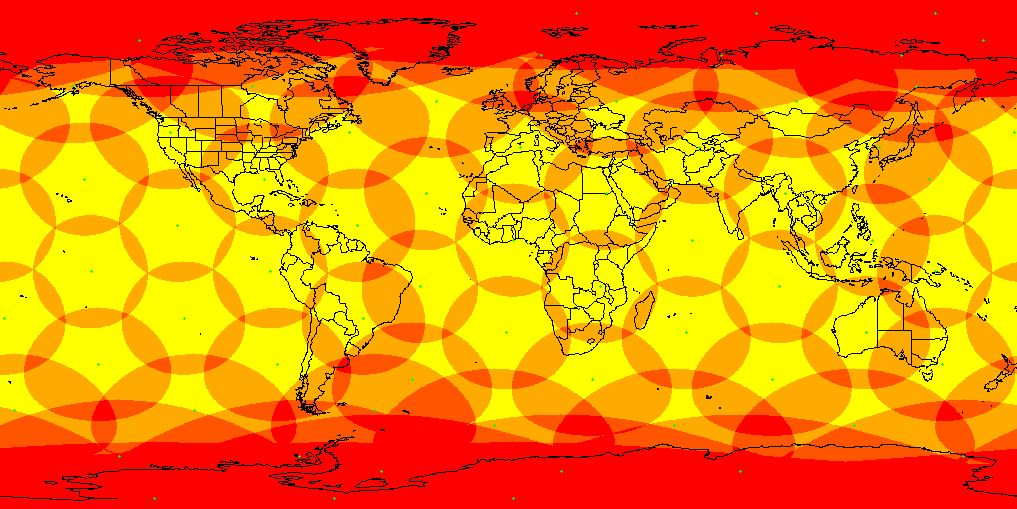
\includegraphics[scale=0.6]{PolarOrbits/Iridium.jpg}
\caption{Distribution of the 66 Iridium constellation satellites. Generated using \cite{Wood2011}}
\end{center}
\end{figure} 
\newpage

\section{The Streets of Coverage Method}
\label{ch:streetscov}
This  Street of Coverage Method is obtained from 
\cite{Chobotov2002}. As you can see in the figure below,
 the relations between angles seen from different satellites can
 be easily computed. The main variables are the following:

\begin{table}[H]
\centering
\begin{tabular}{|c|l|}
\hline
\multicolumn{2}{|c|}{Streets of Coverage Method Variables}     \\ \hline
$$N$$              & Number of Satellites                      \\ \hline
$n_{p}$            & Number of Planes                          \\ \hline
$N_{pp}$           & Number of Satellites per plane            \\ \hline
$$S$$              & Separation between satellites of the same plane \\ \hline
$$D$$              & General space between planes {[}º{]}      \\ \hline
$D_{0}$            & Space between antiparallel planes {[}º{]} \\ \hline
$\varepsilon$      & Elevation angle {[}º{]}                   \\ \hline
$\lambda_{street}$ & Street of coverage Width {[}º{]}          \\ \hline
$\lambda_{max}$    & Maximum footprint Radius {[}º{]}          \\ \hline
\end{tabular}
\caption{Streets of Coverage Method main variables}
\end{table}  

\begin{figure}[H]
\begin{center}
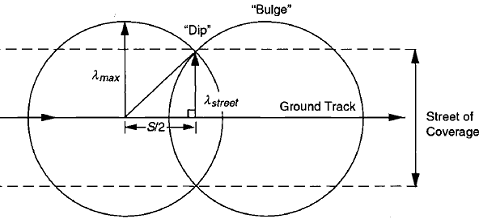
\includegraphics[scale=0.7]{PolarOrbits/planestreet.png}
\caption{Single plain street of coverage. The footprints of the satellites superpose leading to a street.\cite{ccar}}
\end{center}
\end{figure}

From the figure it can be inferred:

$$S < 2\lambda_{max}$$
$$cos(\lambda_{street}) = cos(\lambda_{street})/cos(S/2)$$

\begin{figure}[H]
\begin{center}
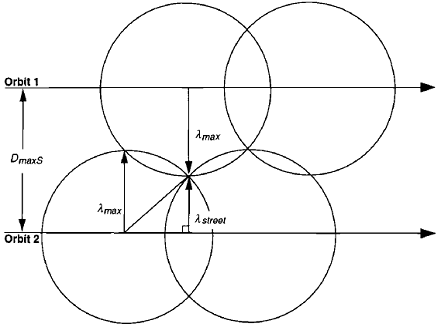
\includegraphics[scale=0.7]{PolarOrbits/planeseps.png}
\caption{Two plains streets of coverage. An optimum phasing needs to be obtained.\cite{ccar}}
\end{center}
\end{figure}

From this point of view, in general:
$$D = \lambda_{street} + \lambda_{max}$$
n
For the antiparallel planes:
$$D_{0} = 2\lambda_{street}$$

And the overall relationship between planes sums:
$$180 = (n_{p}-1)D + D_{0}$$

The algorithm for computing the Streets of Coverage Results is defined in the following way:

\begin{center}
Inputs: Height, elevation, inclination... 
$\rightarrow$
$\lambda_{max}$
$\rightarrow$
$N_{pp}=\left \lceil \frac{360}{2 \lambda_{max}}  \right \rceil$
$\rightarrow$
\newline
$S=360/N_{pp}$
$\rightarrow$
$\lambda_{street}$
$\rightarrow$
$n_{p}$
$\rightarrow$
$N=N_{pp}*n_{p}$
\end{center}

\subsection{Results of Streets of Coverage}
A MATLAB routine has been designed to compute the previously described algorithm. In this conceptual design phase, different heights are computed in order to see the evolution of the number of satellites.

\subsubsubsection*{General Solution}
The program in runned in a broad range of parameters to see the evolution of the number of satellites. As it can be predicted, as the height increases the number of satellites is reduced. The reason is that the footprint of the satellites increases with the height. In addition, as the minimum elevation over the horizon to contact the satellites is reduced, the number of satellites is also reduced for the same reason.

\begin{figure}[H]
\begin{center}
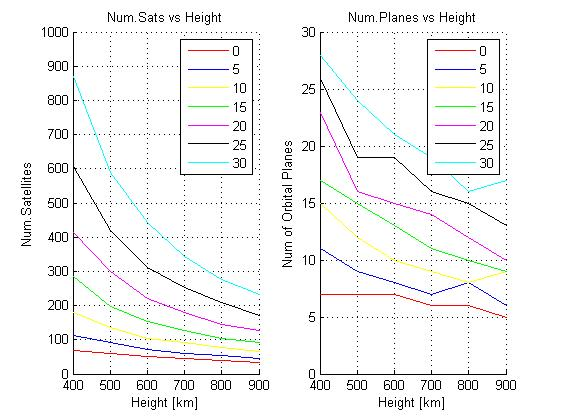
\includegraphics[scale=0.7]{PolarOrbits/GeneralResults.jpg}
\caption{Variation of number of satellites for different heights and elevation angles}
\end{center}
\end{figure}

\subsubsubsection*{Detailed Solution}
Given the previously justified assumptions, the same simulation is computed for a more reasonable range of results. In this case, the elevation is set as: $$\varepsilon = 20º$$.

\begin{figure}[H]
\begin{center}
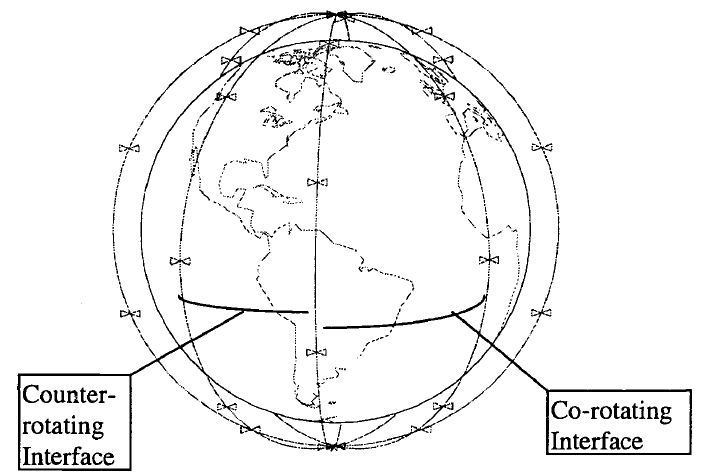
\includegraphics[scale=0.7]{PolarOrbits/Polar.jpg}
\caption{Variation of number of satellites for different heights between 500 and 600km.}
\end{center}
\end{figure}

\subsubsubsection*{Conclusion}
The computation and the design of this constellation requires small computational and conceptual effort. However, the number of satellites and planes is greater than expected. Even though the technical complexity can be reduced, the availability of small launchers to reach this particularly inclined orbit is also small. In conclusion, more constellation configurations need to be assessed to compare and select the most feasible one.

%\bibliographystyle{unsrt}
%\bibliography{forouzan,Secretariat2014,TC,tmsynch,OrbitalMechanics
%\end{document}